\documentclass[a4paper,norsk]{article}
\usepackage{preamble}
\usepackage{tabu}

\begin{document}
\maketitle

\section*{Problem 1}

In this exercise we are faced with a problem on the domain $\Omega = (0,1)^2$
\begin{align}
&-\nabla u = f\text{ in } \Omega \\
&\text{u = 0 for x = 0 and x = 1} \\
&\frac{\partial u}{\partial n} = 0 \text{ for } y = 0 \text{ and } y = 1
\end{align}

We know that the analytical solution is on the form
\begin{align*}
u(x,y) = sin(k \pi x) cos(l \pi y)
\end{align*}

\subsection*{Exercise A}
Given \[ u(x,y) = sin(k \pi x)cos(l \pi y) \] We can calculate the $H^p$ norm as defined
in the lecture notes \textit{Definition 2.13} as follows

\[||u||_{H^p} = \sqrt{ \sum_{|\alpha| \leq p} \int_\Omega |\partial^{\alpha} v|^2 dx }   \]

We restrict $k,l$ to be whole numbers $k,l \in \mathbb{Z} $ \\
To find some sort of relation of this sum, we first look at the case $\alpha = 0$
\begin{align*}
\int_0^1 \int_0^1 sin^2(k \pi x) cos^2(l \pi y) dx dy  \\ \\
-\frac{(-2k\pi + sin(2 k \pi))(2 l \pi + sin(2 l \pi))  }{16 k l \pi^2}   = \frac{1}{4}
\end{align*}

Exploiting the relations which will appear in the integration of the derivatives
\begin{align*}
\int_0^1 sin^2(k \pi x) dx = \frac{1}{2} \hspace{5mm} \int_0^1 cos^2(k \pi x) dx = \frac{1}{2}
\end{align*}

We can express the $H^p$ norm as the sum
\begin{align*}
H^p = \sqrt{\frac{1}{4} \sum_0^p ((k \pi)^2 + (l \pi)^2 )^p  }
\end{align*}


\subsection*{Exericse B}
In this exercise we were to calculate the $L_2$ and $H^1$ errors form our numerical experiments.
The experiments were calculated on a unit squaremesh for $\frac{1}{h} = [8, 16, 32, 64]$.
I chose to limit my exploration of errors to the case
where $k = l = [1, 10, 100]$. I still think this limitation shows the significant trends
we are supposed to look at. My program yields the following output.

\newpage
\begin{lstlisting}[style=terminal]
###########################################################

#-------------------- 1 degree elements -----------------#

###########################################################


###########################################################

#----------------------- L2 Norm ---------------------#

=============  ========  ========  ======  ======
Values of N           8        16      32      64
=============  ========  ========  ======  ======
k_l = 1          0.0328    0.0085  0.0021  0.0005
k_1 = 10         0.6671    0.3655  0.1782  0.0549
k_l = 100      159.356   246.862   2.6969  3.5888
=============  ========  ========  ======  ======

#----------------------- H1 Norm ---------------------#

=============  =========  =========  ========  ========
Values of N            8         16        32        64
=============  =========  =========  ========  ========
k_l = 1           0.4366     0.2182    0.1091    0.0545
k_1 = 10         26.4815    17.5464   10.6024    5.4399
k_l = 100      3226.29    4686.2     376.364   540.467
=============  =========  =========  ========  ========

###########################################################

#-------------------- Linear Approximation ---------------#


                       Norm = L2     k_l = 1
                     alpha = 1.9804, Constant = 2.0308

Errornorm (u-u_h) < C*h^(alpha) is True for N = 8
Errornorm (u-u_h) < C*h^(alpha) is True for N = 16
Errornorm (u-u_h) < C*h^(alpha) is True for N = 32
Errornorm (u-u_h) < C*h^(alpha) is True for N = 64

                       Norm = H1     k_l = 1
                     alpha = 1.0004, Constant = 3.4954

Errornorm (u-u_h) < C*h^(alpha) is True for N = 8
Errornorm (u-u_h) < C*h^(alpha) is True for N = 16
Errornorm (u-u_h) < C*h^(alpha) is True for N = 32
Errornorm (u-u_h) < C*h^(alpha) is True for N = 64
\end{lstlisting}
\newpage
\begin{lstlisting}[style=terminal]
###########################################################

#-------------------- 2 degree elements -----------------#

###########################################################


###########################################################

#----------------------- L2 Norm ---------------------#

=============  ========  =======  ======  ======
Values of N           8       16      32      64
=============  ========  =======  ======  ======
k_l = 1          0.0006   0.0001  0       0
k_1 = 10         0.4356   0.0896  0.0102  0.0011
k_l = 100      293.246   90.4749  4.7223  1.471
=============  ========  =======  ======  ======

#----------------------- H1 Norm ---------------------#

=============  =========  =========  ========  ========
Values of N            8         16        32        64
=============  =========  =========  ========  ========
k_l = 1           0.0332     0.0084    0.0021    0.0005
k_1 = 10         19.1245     6.9203    1.978     0.5184
k_l = 100      5321.28    1648.5     689.092   288.597
=============  =========  =========  ========  ========

###########################################################

#-------------------- Linear Approximation ---------------#


                       Norm = L2     k_l = 1
                     alpha = 3.0154, Constant = 0.2989

Errornorm (u-u_h) < C*h^(beta) is True for N = 8
Errornorm (u-u_h) < C*h^(beta) is True for N = 16
Errornorm (u-u_h) < C*h^(beta) is True for N = 32
Errornorm (u-u_h) < C*h^(beta) is True for N = 64

                       Norm = H1     k_l = 1
                     alpha = 1.9923, Constant = 2.0955

Errornorm (u-u_h) < C*h^(alpha) is True for N = 8
Errornorm (u-u_h) < C*h^(alpha) is True for N = 16
Errornorm (u-u_h) < C*h^(alpha) is True for N = 32
Errornorm (u-u_h) < C*h^(alpha) is True for N = 64

\end{lstlisting}
\newpage

From the output we observe that both the $L_2$ and $H^1$ norms are increasing
for some chosen point N.\\
For the $L_2$ case the reason for the increasing values is because of the increasing
wavenumber in the analytical solution.  Since the solution has a period of $ \frac{-2 \pi}{k} $ in x
and $\frac{-2\pi}{l}$ in y, we aren't able to represent the solution correctly due to lack of number of elements
for increasing k and l. \\
For the $H_1$ case we would expect increasing $H_1$ values because the oscillating solution, will
result in higher values of the derivative. Hence we would expect higher values for the $H_1$ norm as k and l increase.

\subsection*{Exericse C}
In this exercise we were to evaluate the following error estimates
\begin{align*}
||u - u_h||_1 &<= C_{\alpha}h^{\alpha} \\
||u - u_h||_0 &<= C_{\beta}h^{\beta}
\end{align*}
by employing the least square method to estimate $\alpha$, $\beta$ and C. Here I have limited the experiments
for $k = l = 1$ because this gives the most reasonable numerical results. \\

From our lecture notes we expect the $L_2$ estimate of the error to yield
an $\alpha$ value one value higher than the order of elements. While the $H_1$ estimate of the error
would give $\beta$ same as the order of elements. \\
From the numerical calculations we get

\begin{center}
\begin{tabular}{ ||c c c c c|| }
    \hline
& $\alpha$ & $\beta$ & $C_{\alpha}$ & $C_{\beta}$ \\
\hline\hline
$P1$ & 1.9804  & 1.0004 & 2.0308 & 3.4954  \\
\hline
$P2$ & 3.0154 & 1.9923 & 0.2989 & 2.0955 \\
\hline
\end{tabular}
\end{center}

The \textit{a priori} estimation of convergence rate seems valid according to my calculations.
From my output I also conclude that the error estimates are valid for the case $k=l=1$
for all number of elements.


\section*{Exercise 2}
We are presented with the following system
\begin{align}
&-\mu \Delta u + u_x= 0 \hspace{2mm} \text{in} \hspace{2mm} \Omega \\
&u = 0 \hspace{2mm} \text{for} \hspace{2mm} x = 0 \\
&u = 1 \hspace{2mm} \text{for} \hspace{2mm} x = 1 \\
&\frac{\partial u}{\partial n} = 0 \text{ for } y = 0 \text{ and } y = 1
\end{align}

\subsection*{Exercise A}
By assuming a solution on the form $u(x,y) = X(x)Y(y)$, we get by insertion
\begin{align*}
-\mu(Y(y)X(x)'' + X(x)Y(y)'') + Y(y)X(x)' = 0 \\
\frac{Y''}{Y} = \frac{X' - \mu X''}{\mu X} = -\lambda^2
\end{align*}

Where $\lambda$ is some arbitrary constant.
Solving for Y we get

\begin{align*}
\lambda Y'' + Y &= 0 \\
Y(y) &= Acos(\sqrt{\lambda} y) + B sin(\sqrt{\lambda}y) \\
Y'(y) &= -A\sqrt{\lambda}sin(\sqrt{\lambda} y) + B\sqrt{\lambda}cos(\sqrt{\lambda} y)
\end{align*}
From the boundary conditions, and by assuming $\lambda \neq 0$ we get

\begin{align*}
Y'(0) &= 0 + B\sqrt{\lambda} = 0 \hspace{2mm} B = 0 \\
Y'(1) = -A\sqrt{\lambda}sin(\sqrt{\lambda}) =0 \\
\lambda = n \pi \hspace{2mm} A = 0
\end{align*}

Assuming $\lambda = 0$ we get a linear solution
\begin{align*}
\frac{Y''}{Y} =  0 \\
Y(y) = Ay + B \hspace{2mm} Y'(0) = A = 0 \\
Y(y) = B
\end{align*}
As we can see, the function of Y is just a consant, which is convenient to set as $B = 1$

Now, focusing on the other function of X for $\lambda = 0$ we get

\begin{align*}
&X' - \mu X''= 0 \\
&X(x) = \frac{C}{\mu}e^{\frac{x}{\mu}} + D \\
&X(0) = \frac{C}{\mu} + D = 0 \hspace{4mm} X(1) = \frac{C}{\mu}e^{\frac{1}{\mu}} + D = 1 \\ \\
&X(x) = \frac{e^{\frac{x}{\mu}} -1}{e^{\frac{1}{\mu}} - 1}
\end{align*}

Hence the analytical solution can be expressed as

\begin{align}
u(x) = \frac{e^{\frac{x}{\mu}} -1}{e^{\frac{1}{\mu}} - 1}
\end{align}

\subsection*{Exercise B}
Running the numerical experiments for values \newline
$\mu = [1, 0.1, 0.01, 0.001, 0.0001]$ \newline
$h = [8, 16, 32, 64]$ \newline

I get the following output

\newpage
\begin{lstlisting}[style=terminal]
###########################################################

#-------------------- 1 degree elements -----------------#

###########################################################


###########################################################

#-------------------- Linear Approximation ---------------#

                 Norm = L2     my = 1
                 alpha = 1.9998, Constant = 0.0897

Errornorm (u-u_h) < C*h^(alpha) is True for N = 8
Errornorm (u-u_h) < C*h^(alpha) is True for N = 16
Errornorm (u-u_h) < C*h^(alpha) is True for N = 32
Errornorm (u-u_h) < C*h^(alpha) is True for N = 64
                 Norm = H1     my = 1
                 alpha = 0.9998, Constant = 0.3001

Errornorm (u-u_h) < C*h^(alpha) is True for N = 8
Errornorm (u-u_h) < C*h^(alpha) is True for N = 16
Errornorm (u-u_h) < C*h^(alpha) is True for N = 32
Errornorm (u-u_h) < C*h^(alpha) is True for N = 64
###########################################################

#----------------------- L2 Norm ---------------------#

=============  ==========  ==========  ==========  ==========
Values of N             8          16          32          64
=============  ==========  ==========  ==========  ==========
my = 1           0.001402    0.000351    8.8e-05     2.2e-05
my = 0.1         0.023754    0.006177    0.001561    0.000391
my = 0.01        0.237934    0.103936    0.038186    0.011259
my = 0.001     nan         nan         nan         nan
my = 0.0001    nan         nan         nan         nan
=============  ==========  ==========  ==========  ==========

#----------------------- H1 Norm ---------------------#

=============  ==========  ==========  ==========  ==========
Values of N             8          16          32          64
=============  ==========  ==========  ==========  ==========
my = 1           0.037521    0.018765    0.009383    0.004692
my = 0.1         0.767086    0.398104    0.201041    0.100777
my = 0.01        7.23835     6.68438     5.00716     2.96949
my = 0.001     nan         nan         nan         nan
my = 0.0001    nan         nan         nan         nan
=============  ==========  ==========  ==========  ==========
\end{lstlisting}
\newpage
\begin{lstlisting}[style=terminal]
###########################################################

#-------------------- 2 degree elements -----------------#

###########################################################


###########################################################

#-------------------- Linear Approximation ---------------#

                 Norm = L2     my = 1
                 alpha = 2.9940, Constant = 0.0058

Errornorm (u-u_h) < C*h^(alpha) is True for N = 8
Errornorm (u-u_h) < C*h^(alpha) is True for N = 16
Errornorm (u-u_h) < C*h^(alpha) is True for N = 32
Errornorm (u-u_h) < C*h^(alpha) is True for N = 64
                 Norm = H1     my = 1
                 alpha = 1.9940, Constant = 0.0378

Errornorm (u-u_h) < C*h^(alpha) is True for N = 8
Errornorm (u-u_h) < C*h^(alpha) is True for N = 16
Errornorm (u-u_h) < C*h^(alpha) is True for N = 32
Errornorm (u-u_h) < C*h^(alpha) is True for N = 64
###########################################################

#----------------------- L2 Norm ---------------------#

=============  ==========  ==========  ==========  ==========
Values of N             8          16          32          64
=============  ==========  ==========  ==========  ==========
my = 1           1.2e-05     1e-06       0           0
my = 0.1         0.002245    0.000304    3.9e-05     5e-06
my = 0.01        0.085126    0.030391    0.007598    0.001326
my = 0.001     nan         nan         nan         nan
my = 0.0001    nan         nan         nan         nan
=============  ==========  ==========  ==========  ==========

#----------------------- H1 Norm ---------------------#

=============  ==========  =========  ==========  ==========
Values of N             8         16          32          64
=============  ==========  =========  ==========  ==========
my = 1           0.000597    0.00015    3.8e-05     9e-06
my = 0.1         0.118321    0.03164    0.008066    0.002028
my = 0.01        5.14048     3.60445    1.70493     0.566126
my = 0.001     nan         nan        nan         nan
my = 0.0001    nan         nan        nan         nan
=============  ==========  =========  ==========  ==========

\end{lstlisting}
\newpage
We observe from the analytical solution (8)
that for lower values of $\mu$, python isn't able to represent the exponential
$exp(\frac{1}{\mu})$. Hence we get values in the output that
python can't produce. \newline
Another consequence is that the diffusion term contributes less to the solution
. The solution change from one of exponential growth to a sudden steep gradient
at the end of the domain. This gives certain effects in the calculated norms as we
decrease the value of $\mu$. This sudden gradient will result some larger errors
which will effect the L2 norm, and ecspecially the H1 norm as we can see from the
output.

\begin{figure}
	\centering
	\caption*{Representation of the calculated solution for $\mu$ = 0.001}
	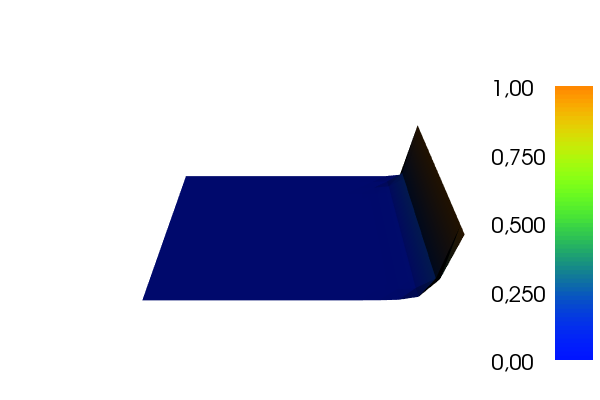
\includegraphics[scale=0.6]{dolfin_plot_2.png}
\end{figure}

\subsection*{Exericse C}
In this exercise we where to evaluate the following error estimates again
\begin{align*}
||u - u_h||_1 &<= C_{\alpha}h^{\alpha} \\
||u - u_h||_0 &<= C_{\beta}h^{\beta}
\end{align*}
by employing least square method to estimate $\alpha$, $\beta$ and C. Here I have limited the experiments
for $\mu = 1$ because this gives the most reasonable numerical results. \\

\begin{center}
\begin{tabular}{ ||c c c c c|| }
    \hline
& $\alpha$ & $\beta$ & $C_{\alpha}$ & $C_{\beta}$ \\
\hline\hline
$P1$ & 1.9998  &  0.9998 & 0.0897 & 0.3001 \\
\hline
$P2$ & 2.9940 & 1.9940 & 0.0058 & 0.0378 \\
\hline
\end{tabular}
\end{center}

Using the same arguments as in exercise 1c, we see that the presented results
as for convergence rates are satisfying.
\newpage
\subsection*{Exericse D}
In this exercise we were to implement the  Streamwise Upwinding
Petrov-Galerkin (SUPG) method. From our lecture notes we know that an
alternative errornorm is presented to obtain better error estimates.
\begin{align*}
||u||_{sd} = \Big(h ||v \cdot \nabla u||^2 +
\mu ||\nabla u ||^2  \Big)^{\frac{1}{2}} \\
||u - u_h || \leq Ch^{\frac{3}{2}} ||u||_2
\end{align*}
Implementing the SUPG method we exchange the ordinary testfunction \textit{V}
for $L = V + \beta v  \nabla V$. This will induce an artificial diffusion term
to the system, which will in fact transform the system to a upwind system from
from a finite difference point of view. My experiments yields.

\newpage
\begin{lstlisting}[style=terminal]
###########################################################

#-------------------- 1 degree elements -----------------#

###########################################################


###########################################################

#-------------------- Linear Approximation ---------------#

                 Norm     my = 1
                 alpha = 0.5159, Constant = 0.1202

###########################################################

#----------------------- L2 Norm ---------------------#

=============  ==========  ==========  ==========  ==========
Values of N             8          16          32          64
=============  ==========  ==========  ==========  ==========
my = 1           0.030251    0.029669    0.029525    0.029489
my = 0.1         0.317615    0.316281    0.315949    0.315866
my = 0.01        0.422485    0.427869    0.428659    0.428674
my = 0.001     nan         nan         nan         nan
my = 0.0001    nan         nan         nan         nan
=============  ==========  ==========  ==========  ==========

#----------------------- H1 Norm ---------------------#

=============  ==========  ==========  ==========  ==========
Values of N             8          16          32          64
=============  ==========  ==========  ==========  ==========
my = 1           0.105669    0.101119    0.099948    0.099653
my = 0.1         1.69142     1.67803     1.67431     1.67336
my = 0.01        5.08569     6.36207     6.79165     6.85168
my = 0.001     nan         nan         nan         nan
my = 0.0001    nan         nan         nan         nan
=============  ==========  ==========  ==========  ==========
\end{lstlisting}
\newpage
\begin{lstlisting}[style=terminal]
#-------------------- 2 degree elements -----------------#

###########################################################


###########################################################

#-------------------- Linear Approximation ---------------#

                 Norm = L2     k_l = 1
                 alpha = -3.1504, Constant = 0.0104

                 Norm = H1     k_l = 1
                 alpha = -1.3418, Constant = 0.7286

###########################################################

#----------------------- L2 Norm ---------------------#

=============  ==========  ==========  ==========  ==========
Values of N             8          16          32          64
=============  ==========  ==========  ==========  ==========
my = 1           0.410669    0.411099    0.425731    0.5872
my = 0.1         0.394629    0.392419    0.391779    0.391889
my = 0.01        0.435901    0.437556    0.437833    0.43755
my = 0.001     nan         nan         nan         nan
my = 0.0001    nan         nan         nan         nan
=============  ==========  ==========  ==========  ==========

#----------------------- H1 Norm ---------------------#

=============  =========  =========  =========  =========
Values of N            8         16         32         64
=============  =========  =========  =========  =========
my = 1          13.5928    27.3796    61.1822   230.86
my = 0.1         5.14402    9.25837   17.9106    36.2078
my = 0.01        5.98764    7.00016    8.17057    9.61022
my = 0.001     nan        nan        nan        nan
my = 0.0001    nan        nan        nan        nan
=============  =========  =========  =========  =========

\end{lstlisting}
\newpage
From our norms, it seems that the SUPG method is not as accurate as the first
implementation. From our print we also observe that the $\alpha $ value for
P1 elements is 0.51, which is totally wrong from the estimated value of $\frac{3}{2}$
from our lecture notes. I have tried several approaches to fix this without luck...

\newpage
\lstinputlisting[style=python]{task1.py}

\newpage
\lstinputlisting[style=python]{task2.py}

\end{document}
